\documentclass[11pt, oneside]{article}
\usepackage{geometry}
\geometry{letterpaper}
\usepackage{graphicx}
\usepackage{amssymb}
\usepackage{amsmath}
\usepackage{tikz}
\usepackage{tikz-qtree}
\usepackage{url}
\usepackage[T1]{fontenc}

\title{SICP Exercise 3.38}
\author{Yuchong Pan}

\begin{document}
\maketitle

\noindent {\bf a.}
\begin{itemize}
    \item Peter, Paul, Mary: $\$100\rightarrow\$110\rightarrow\$90\rightarrow\$45$;
    \item Peter, Mary, Paul: $\$100\rightarrow\$110\rightarrow\$55\rightarrow\$35$;
    \item Paul, Peter, Mary: $\$100\rightarrow\$80\rightarrow\$90\rightarrow\$45$;
    \item Paul, Mary, Peter: $\$100\rightarrow\$80\rightarrow\$40\rightarrow\$50$;
    \item Mary, Paul, Peter: $\$100\rightarrow\$50\rightarrow\$30\rightarrow\$40$;
    \item Mary, Peter, Paul: $\$100\rightarrow\$50\rightarrow\$60\rightarrow\$40$.
\end{itemize}

\medskip

\noindent {\bf b.} If the system allows the processors to be interleaved, then possible values that could be produced are \$100, \$90, \$80, \$60, \$55, \$50, \$40, and \$30.

\begin{center}
    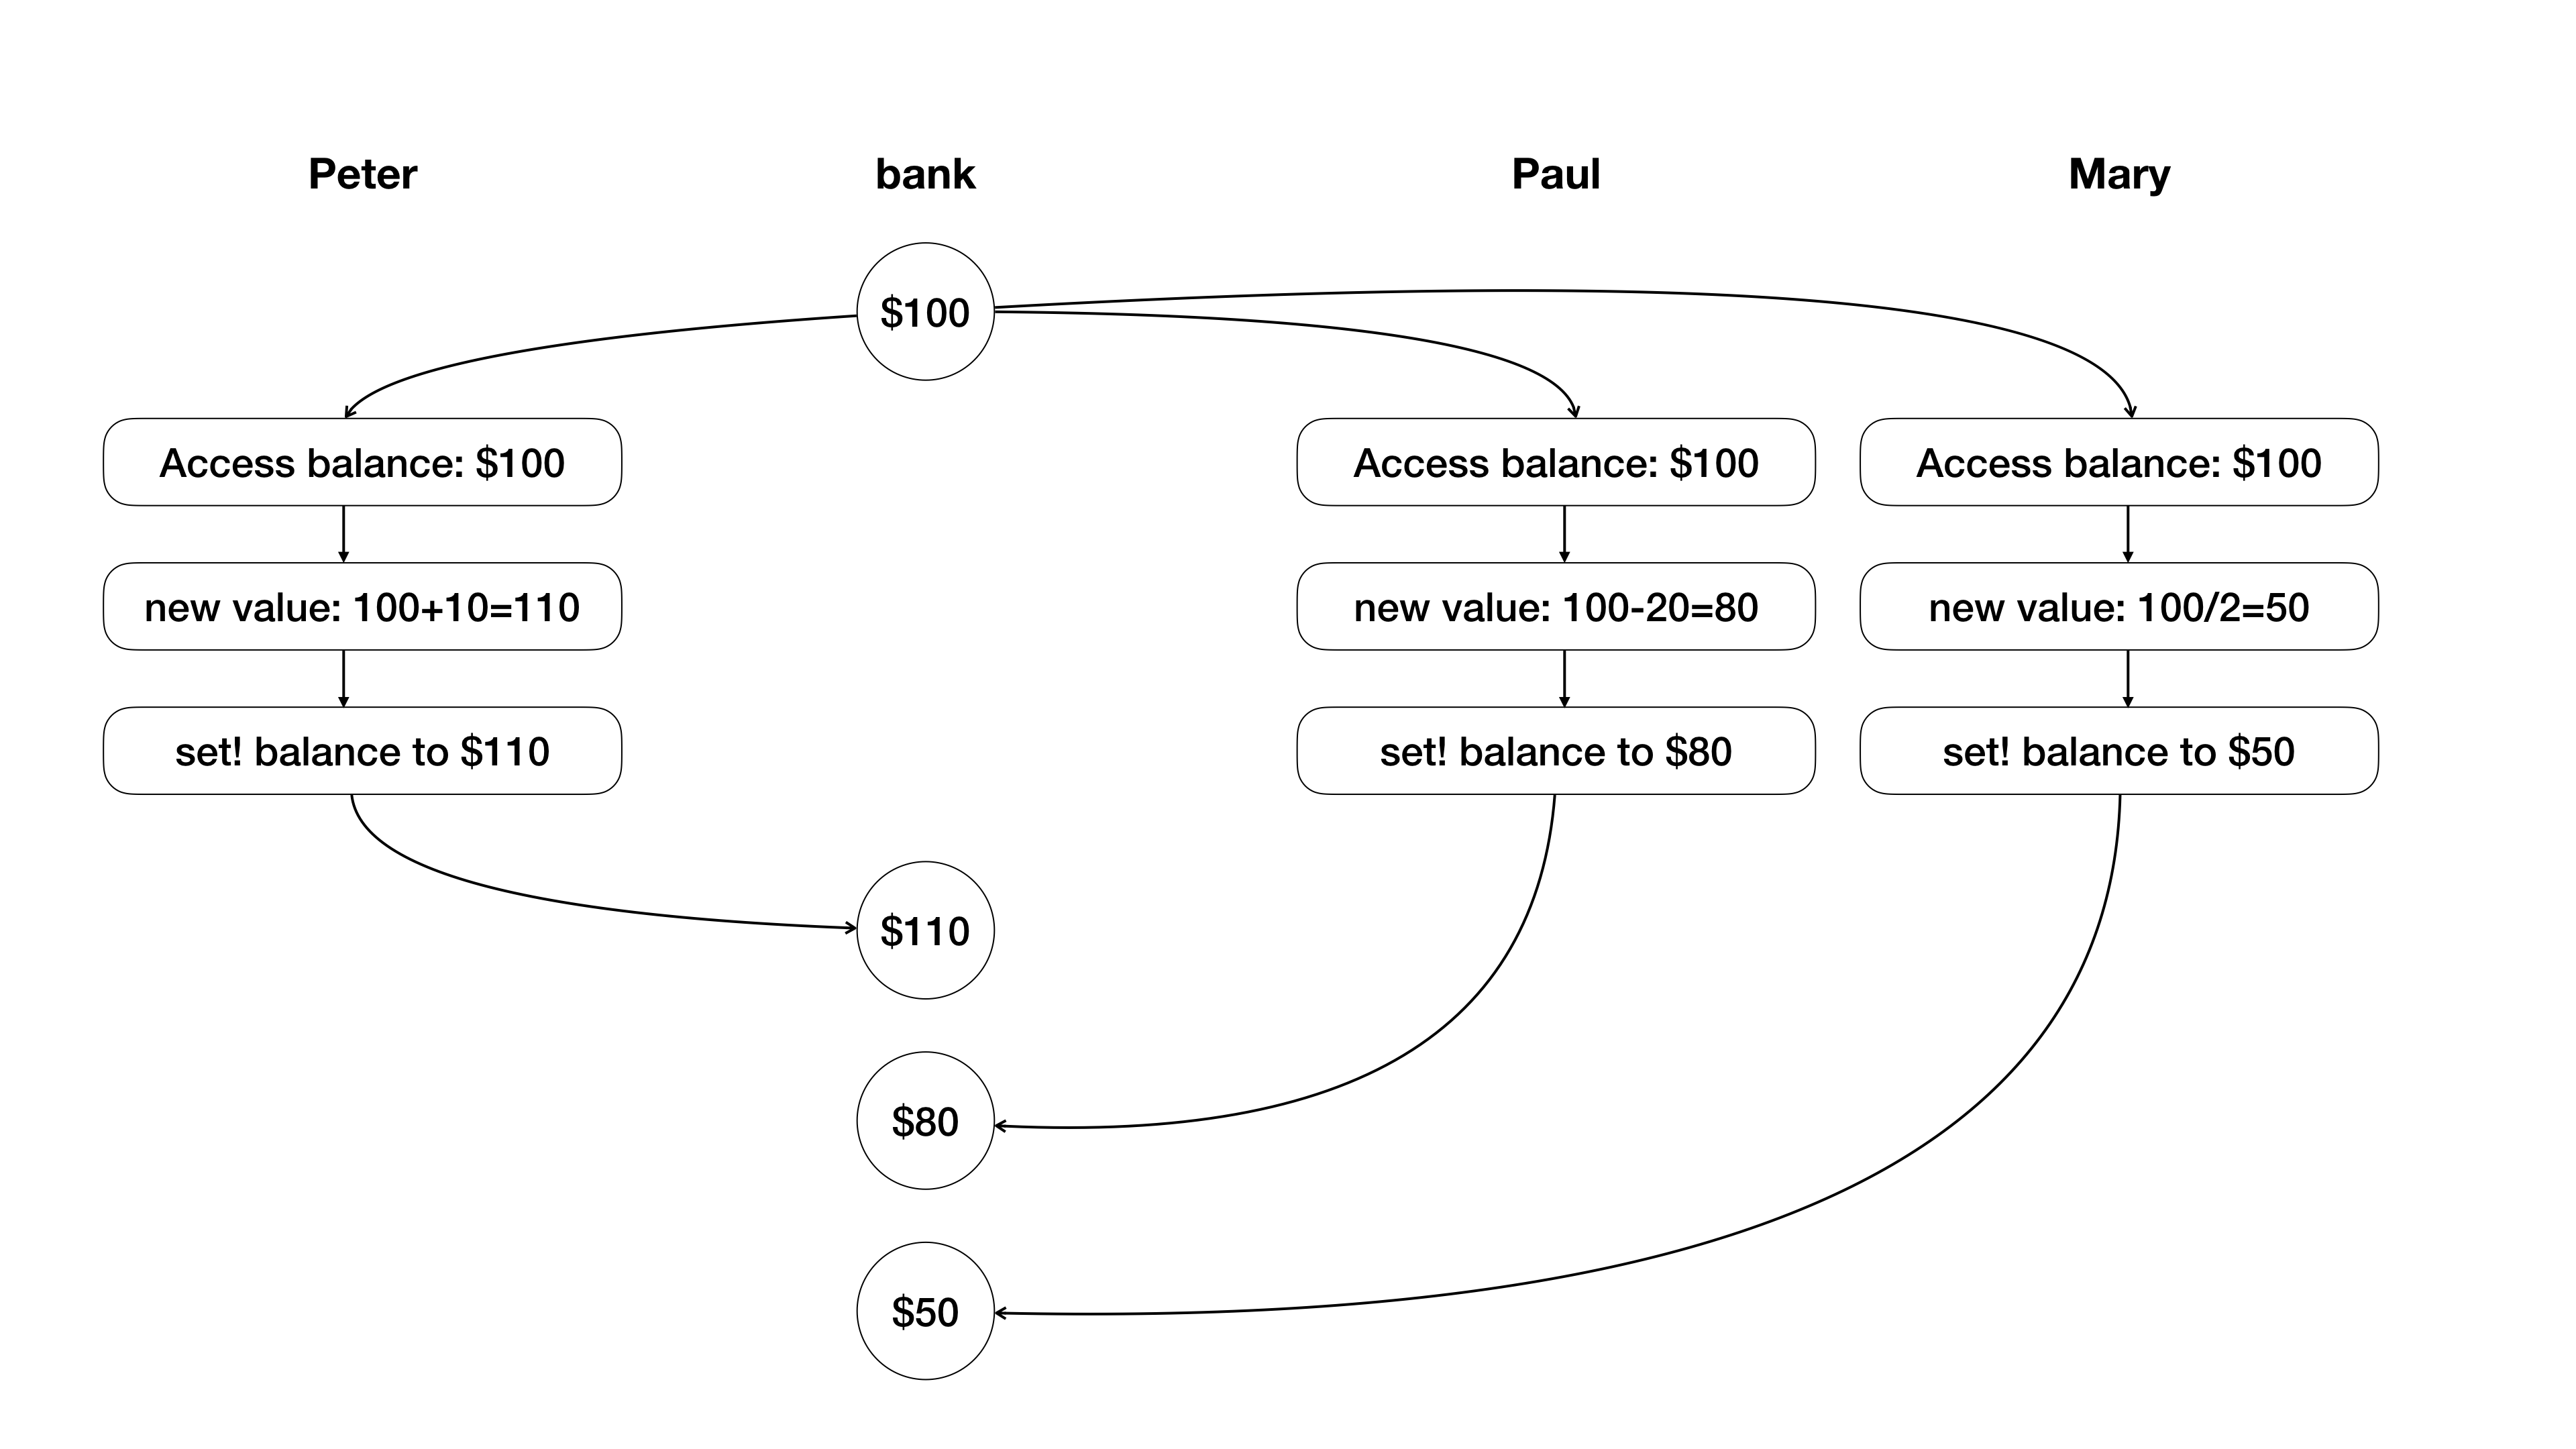
\includegraphics[width=.8\textwidth,height=.8\textheight,keepaspectratio]{1.png}
\end{center}

\begin{center}
    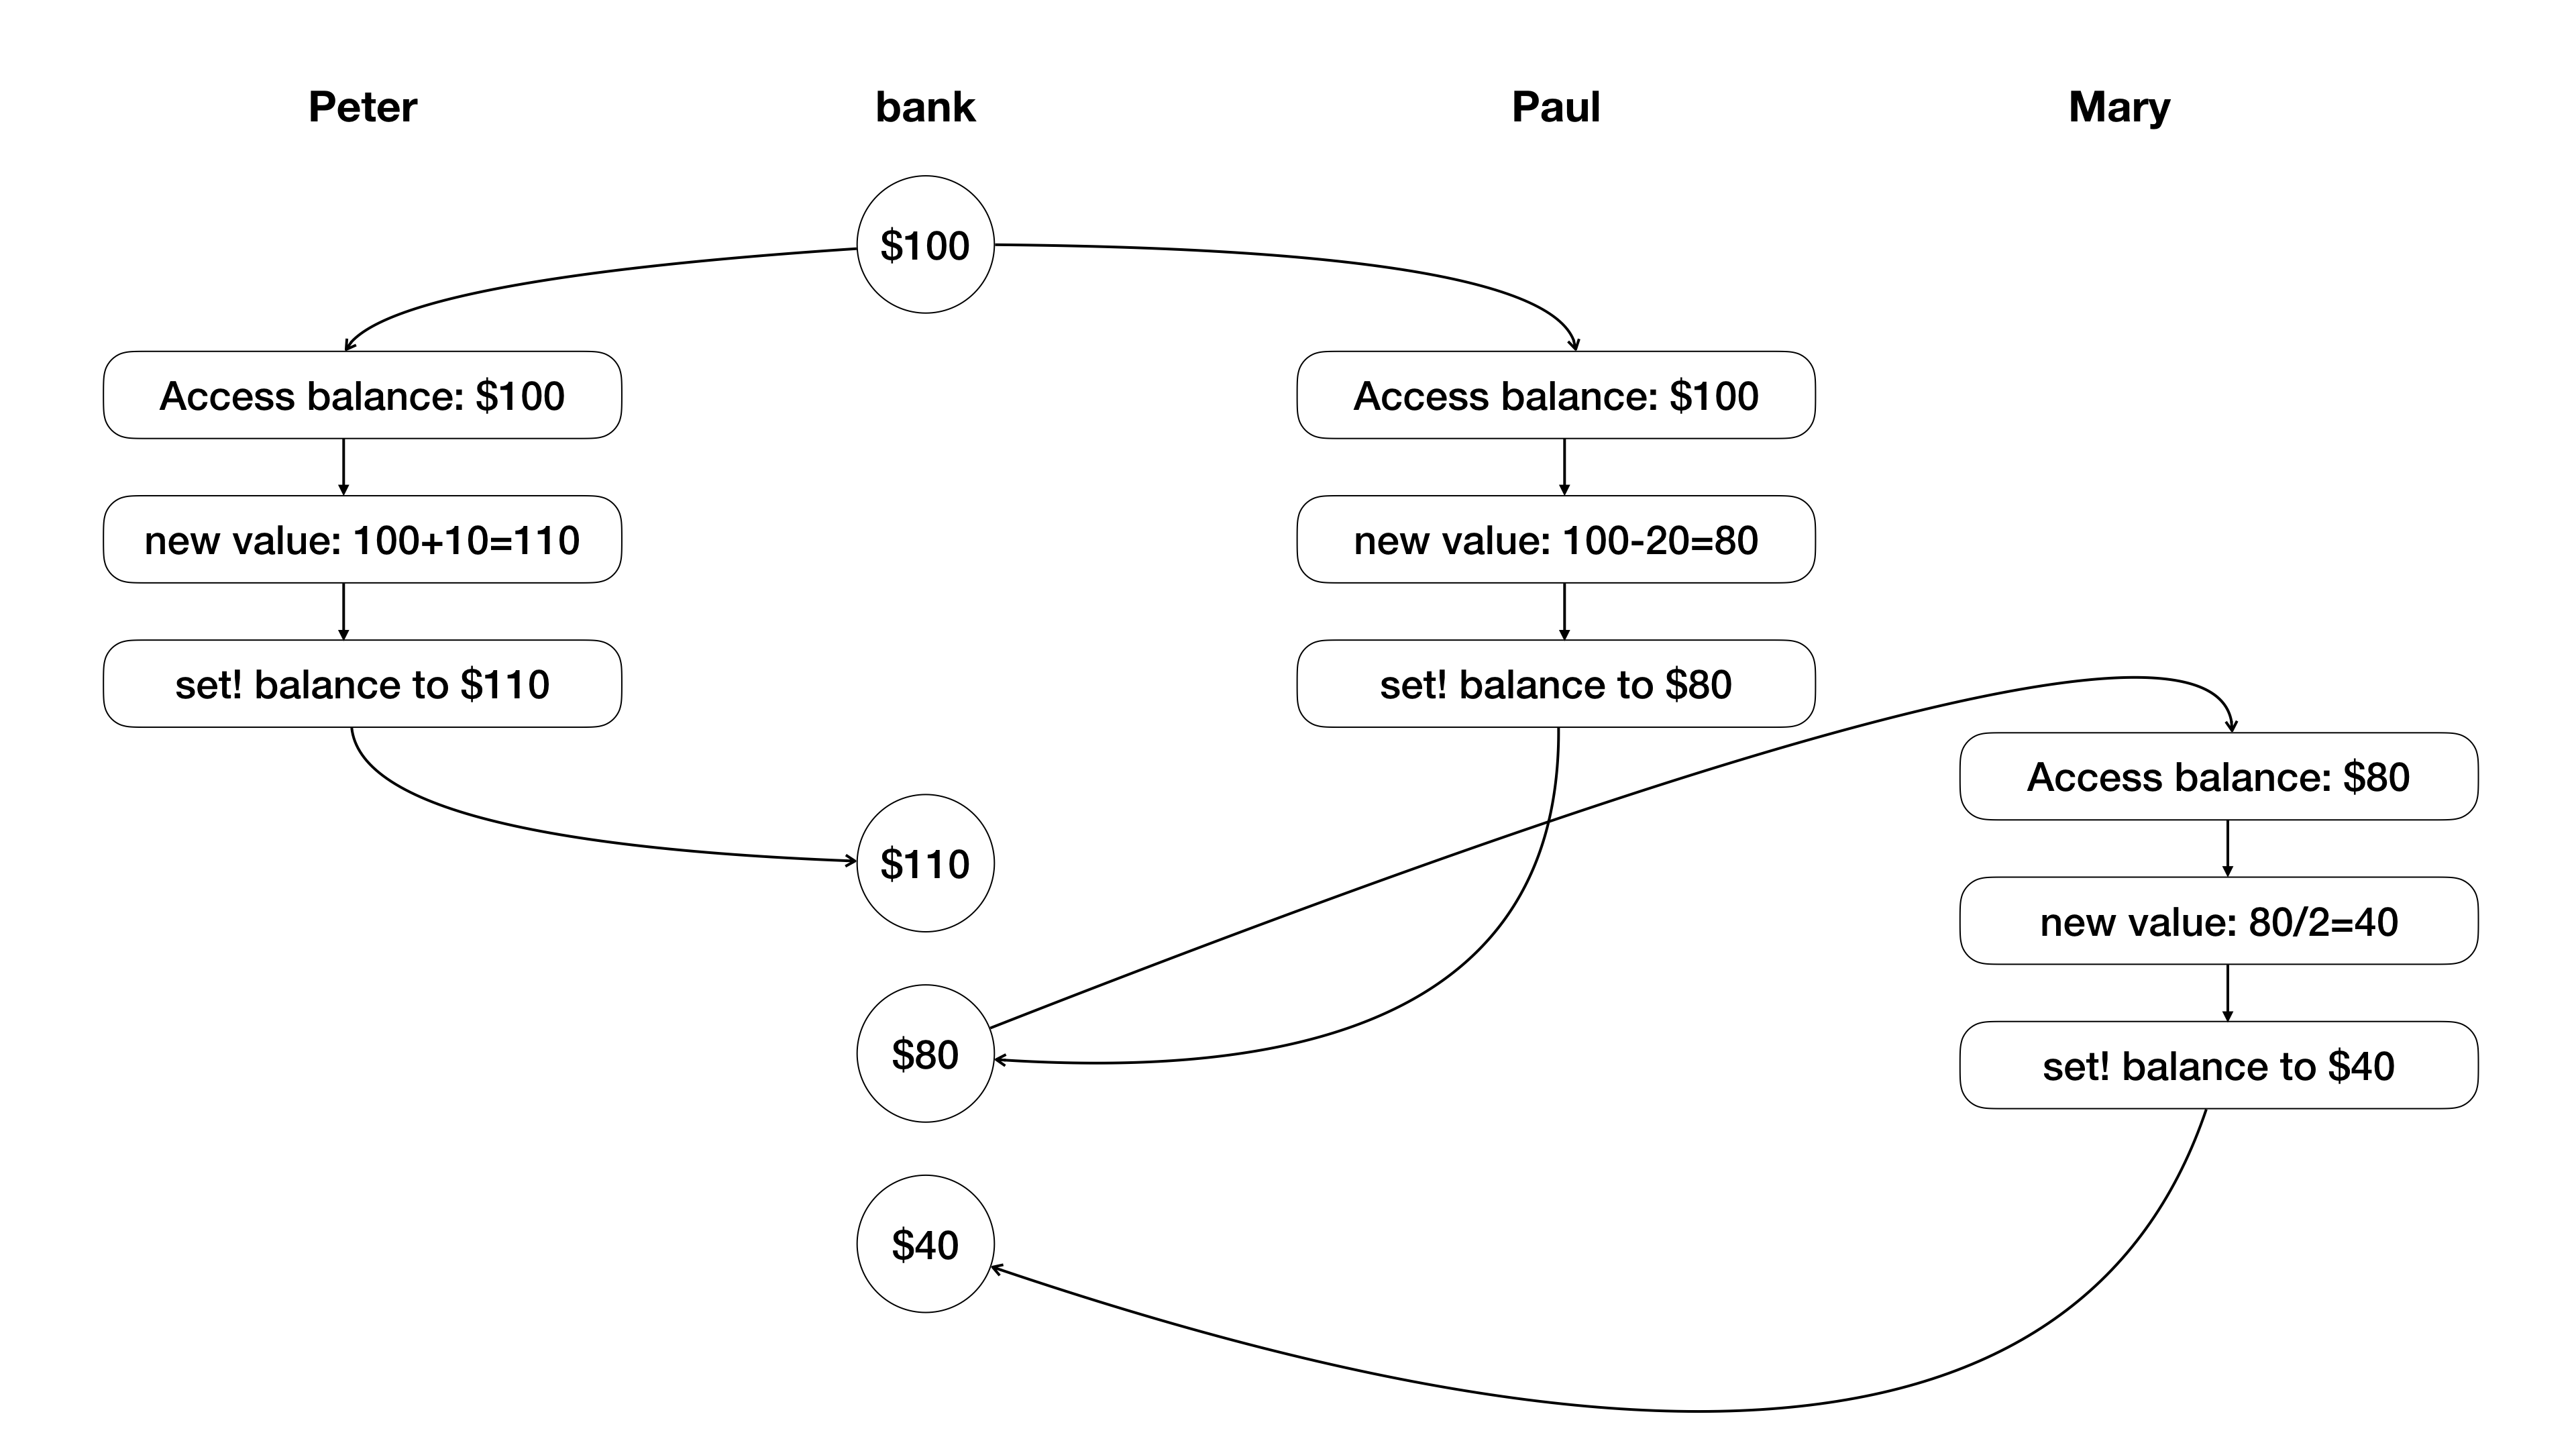
\includegraphics[width=.8\textwidth,height=.8\textheight,keepaspectratio]{2.png}
\end{center}

\begin{center}
    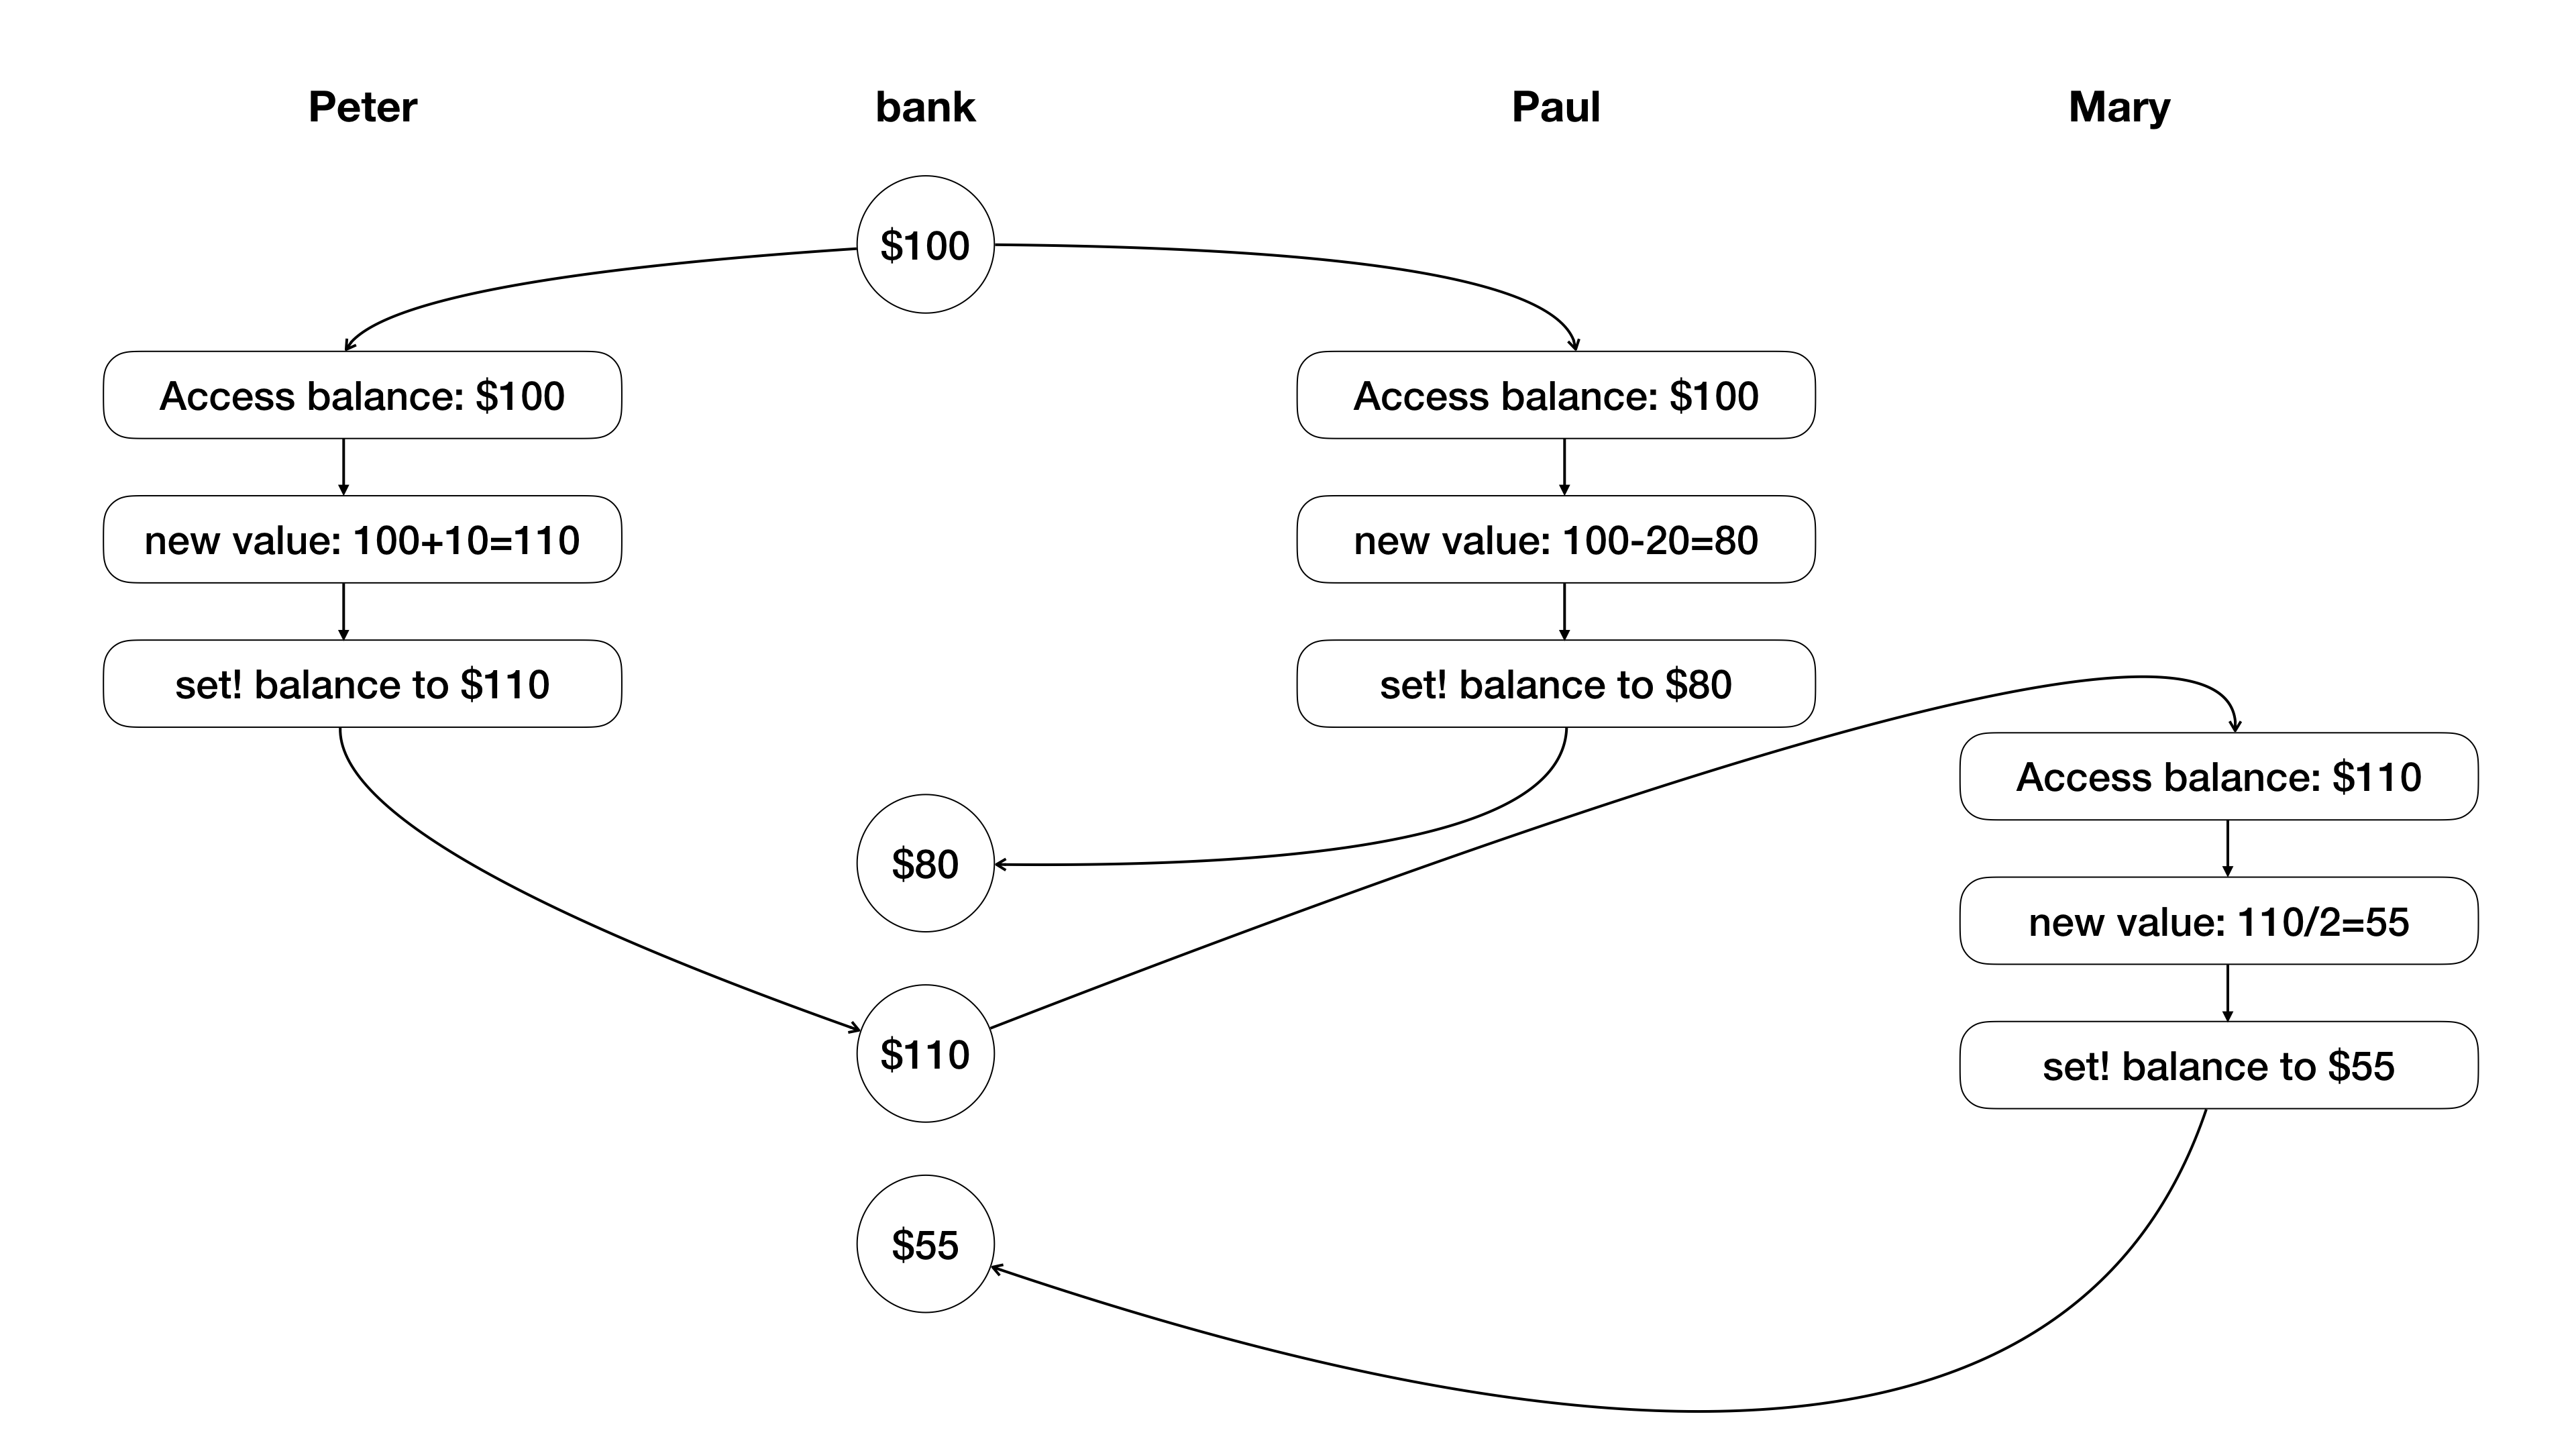
\includegraphics[width=.8\textwidth,height=.8\textheight,keepaspectratio]{3.png}
\end{center}

\begin{center}
    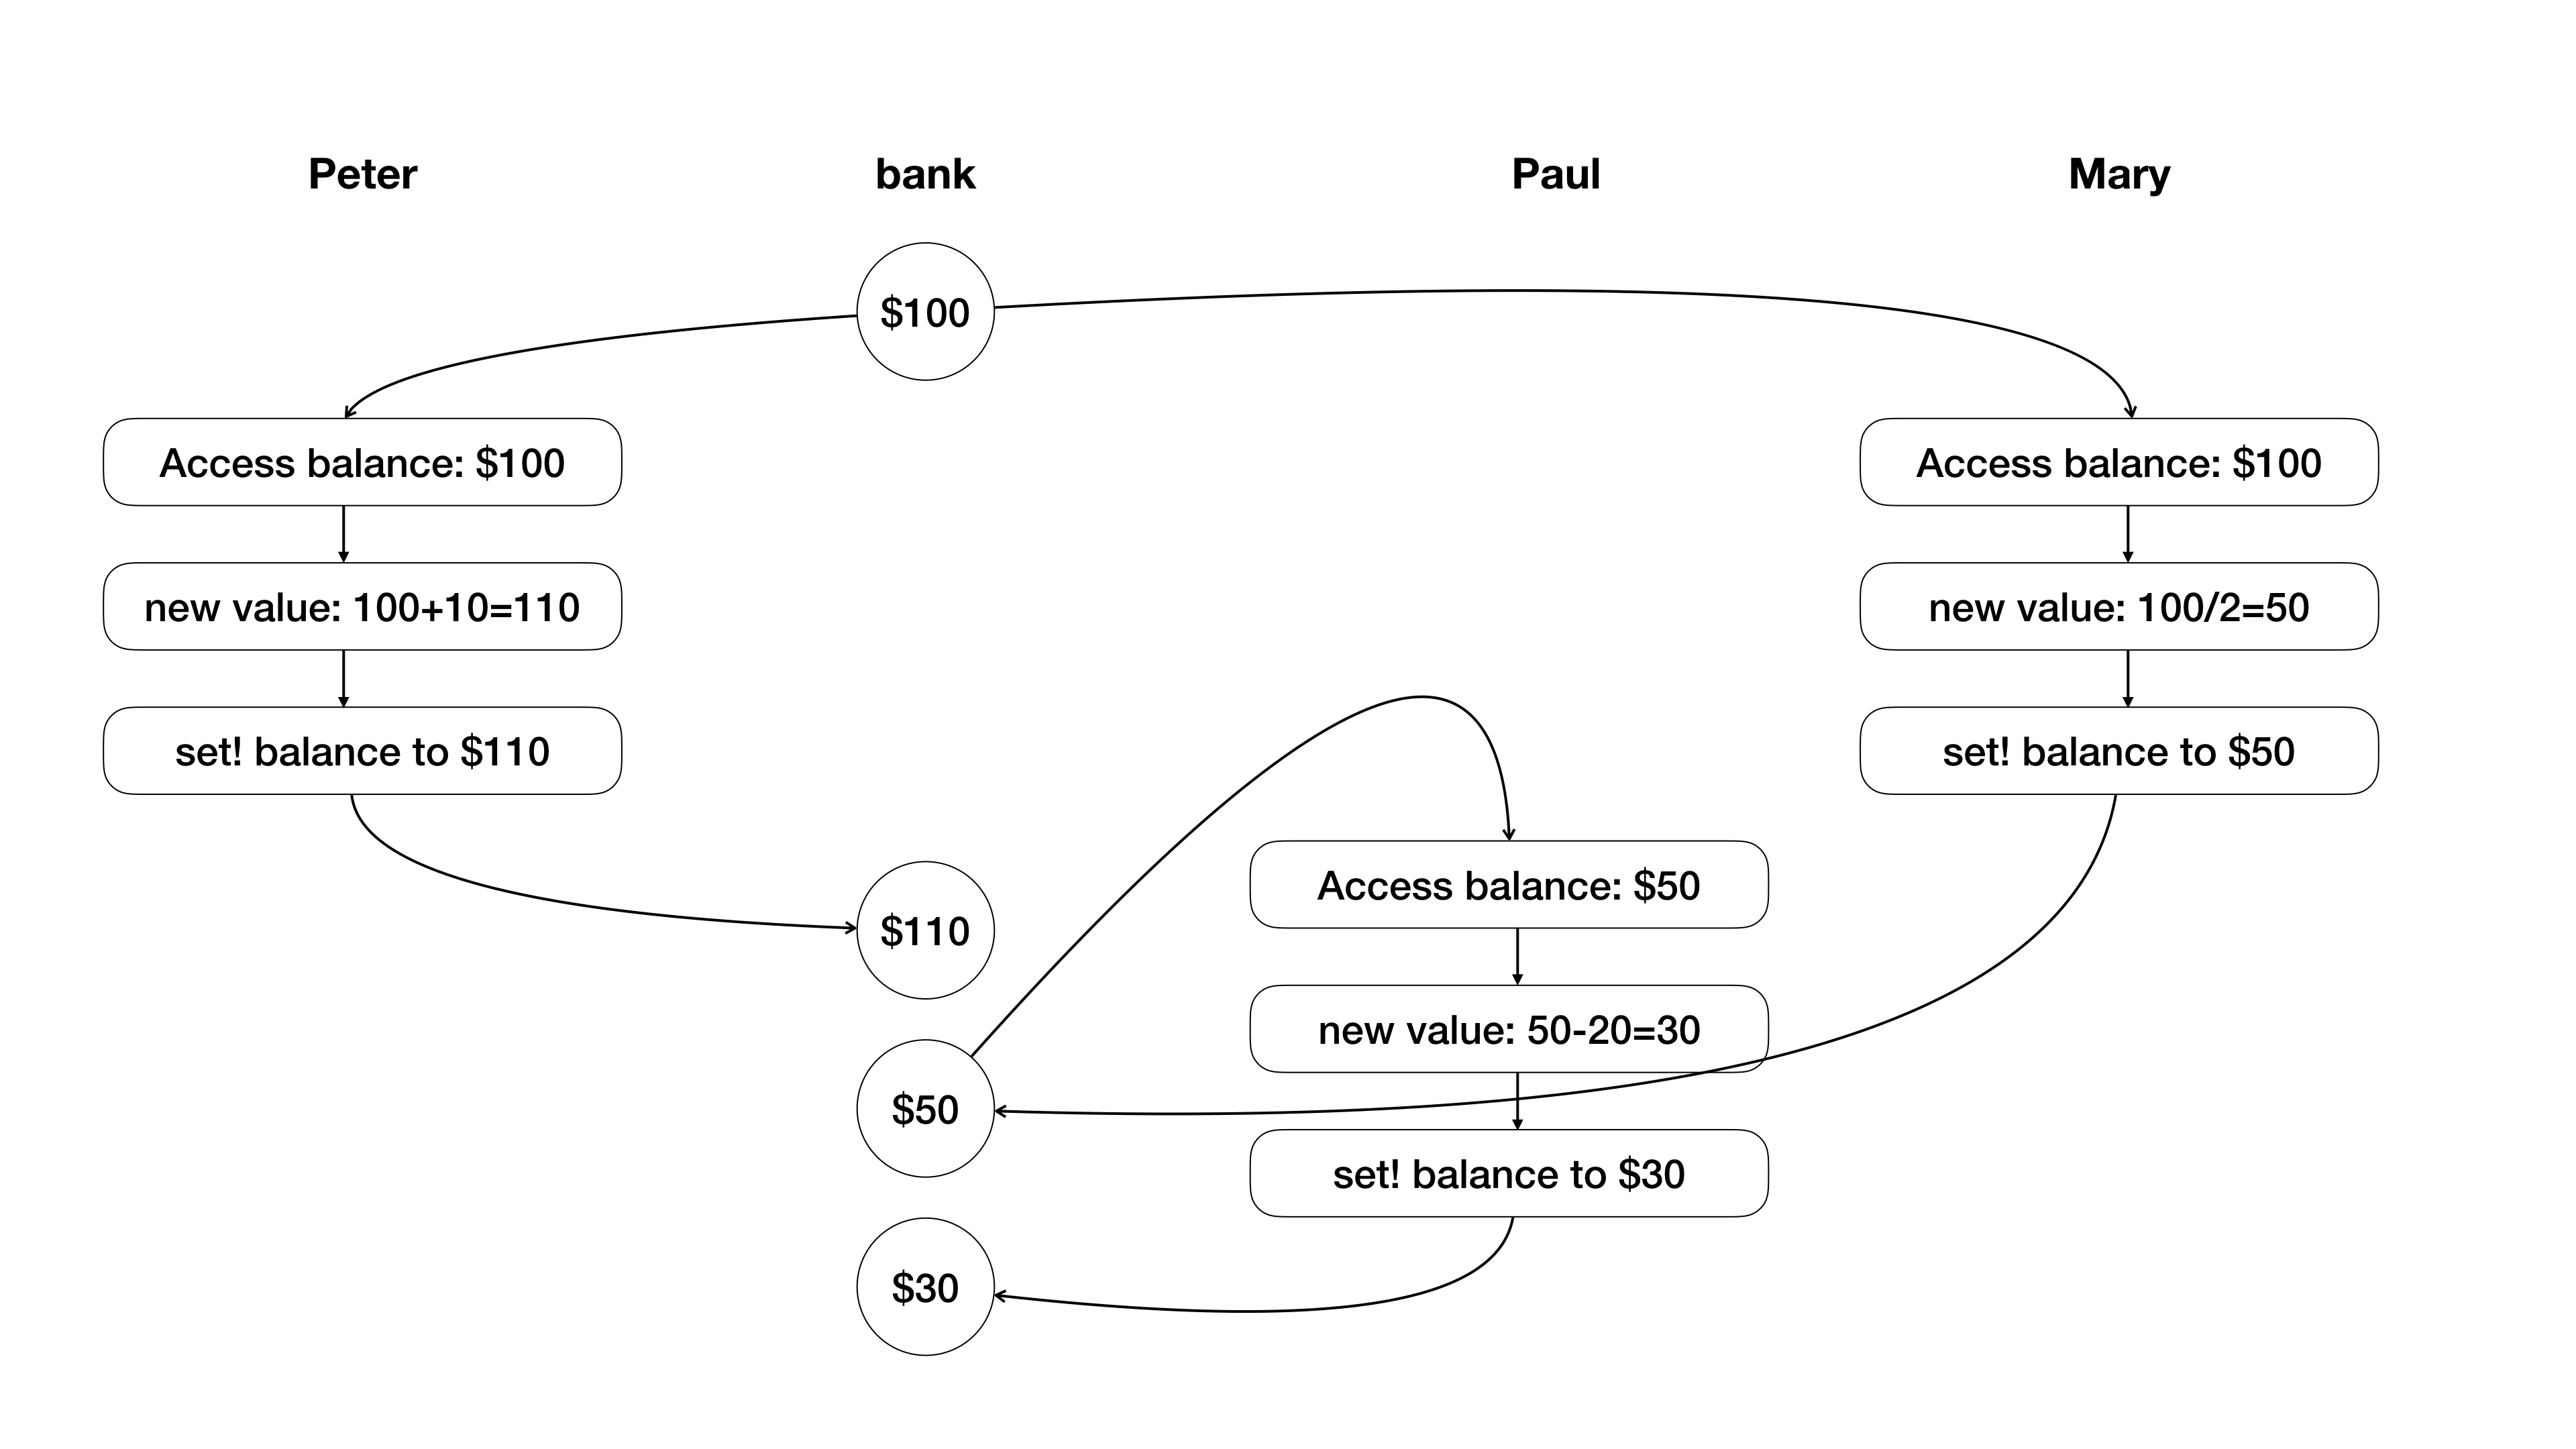
\includegraphics[width=.8\textwidth,height=.8\textheight,keepaspectratio]{4.png}
\end{center}

\begin{center}
    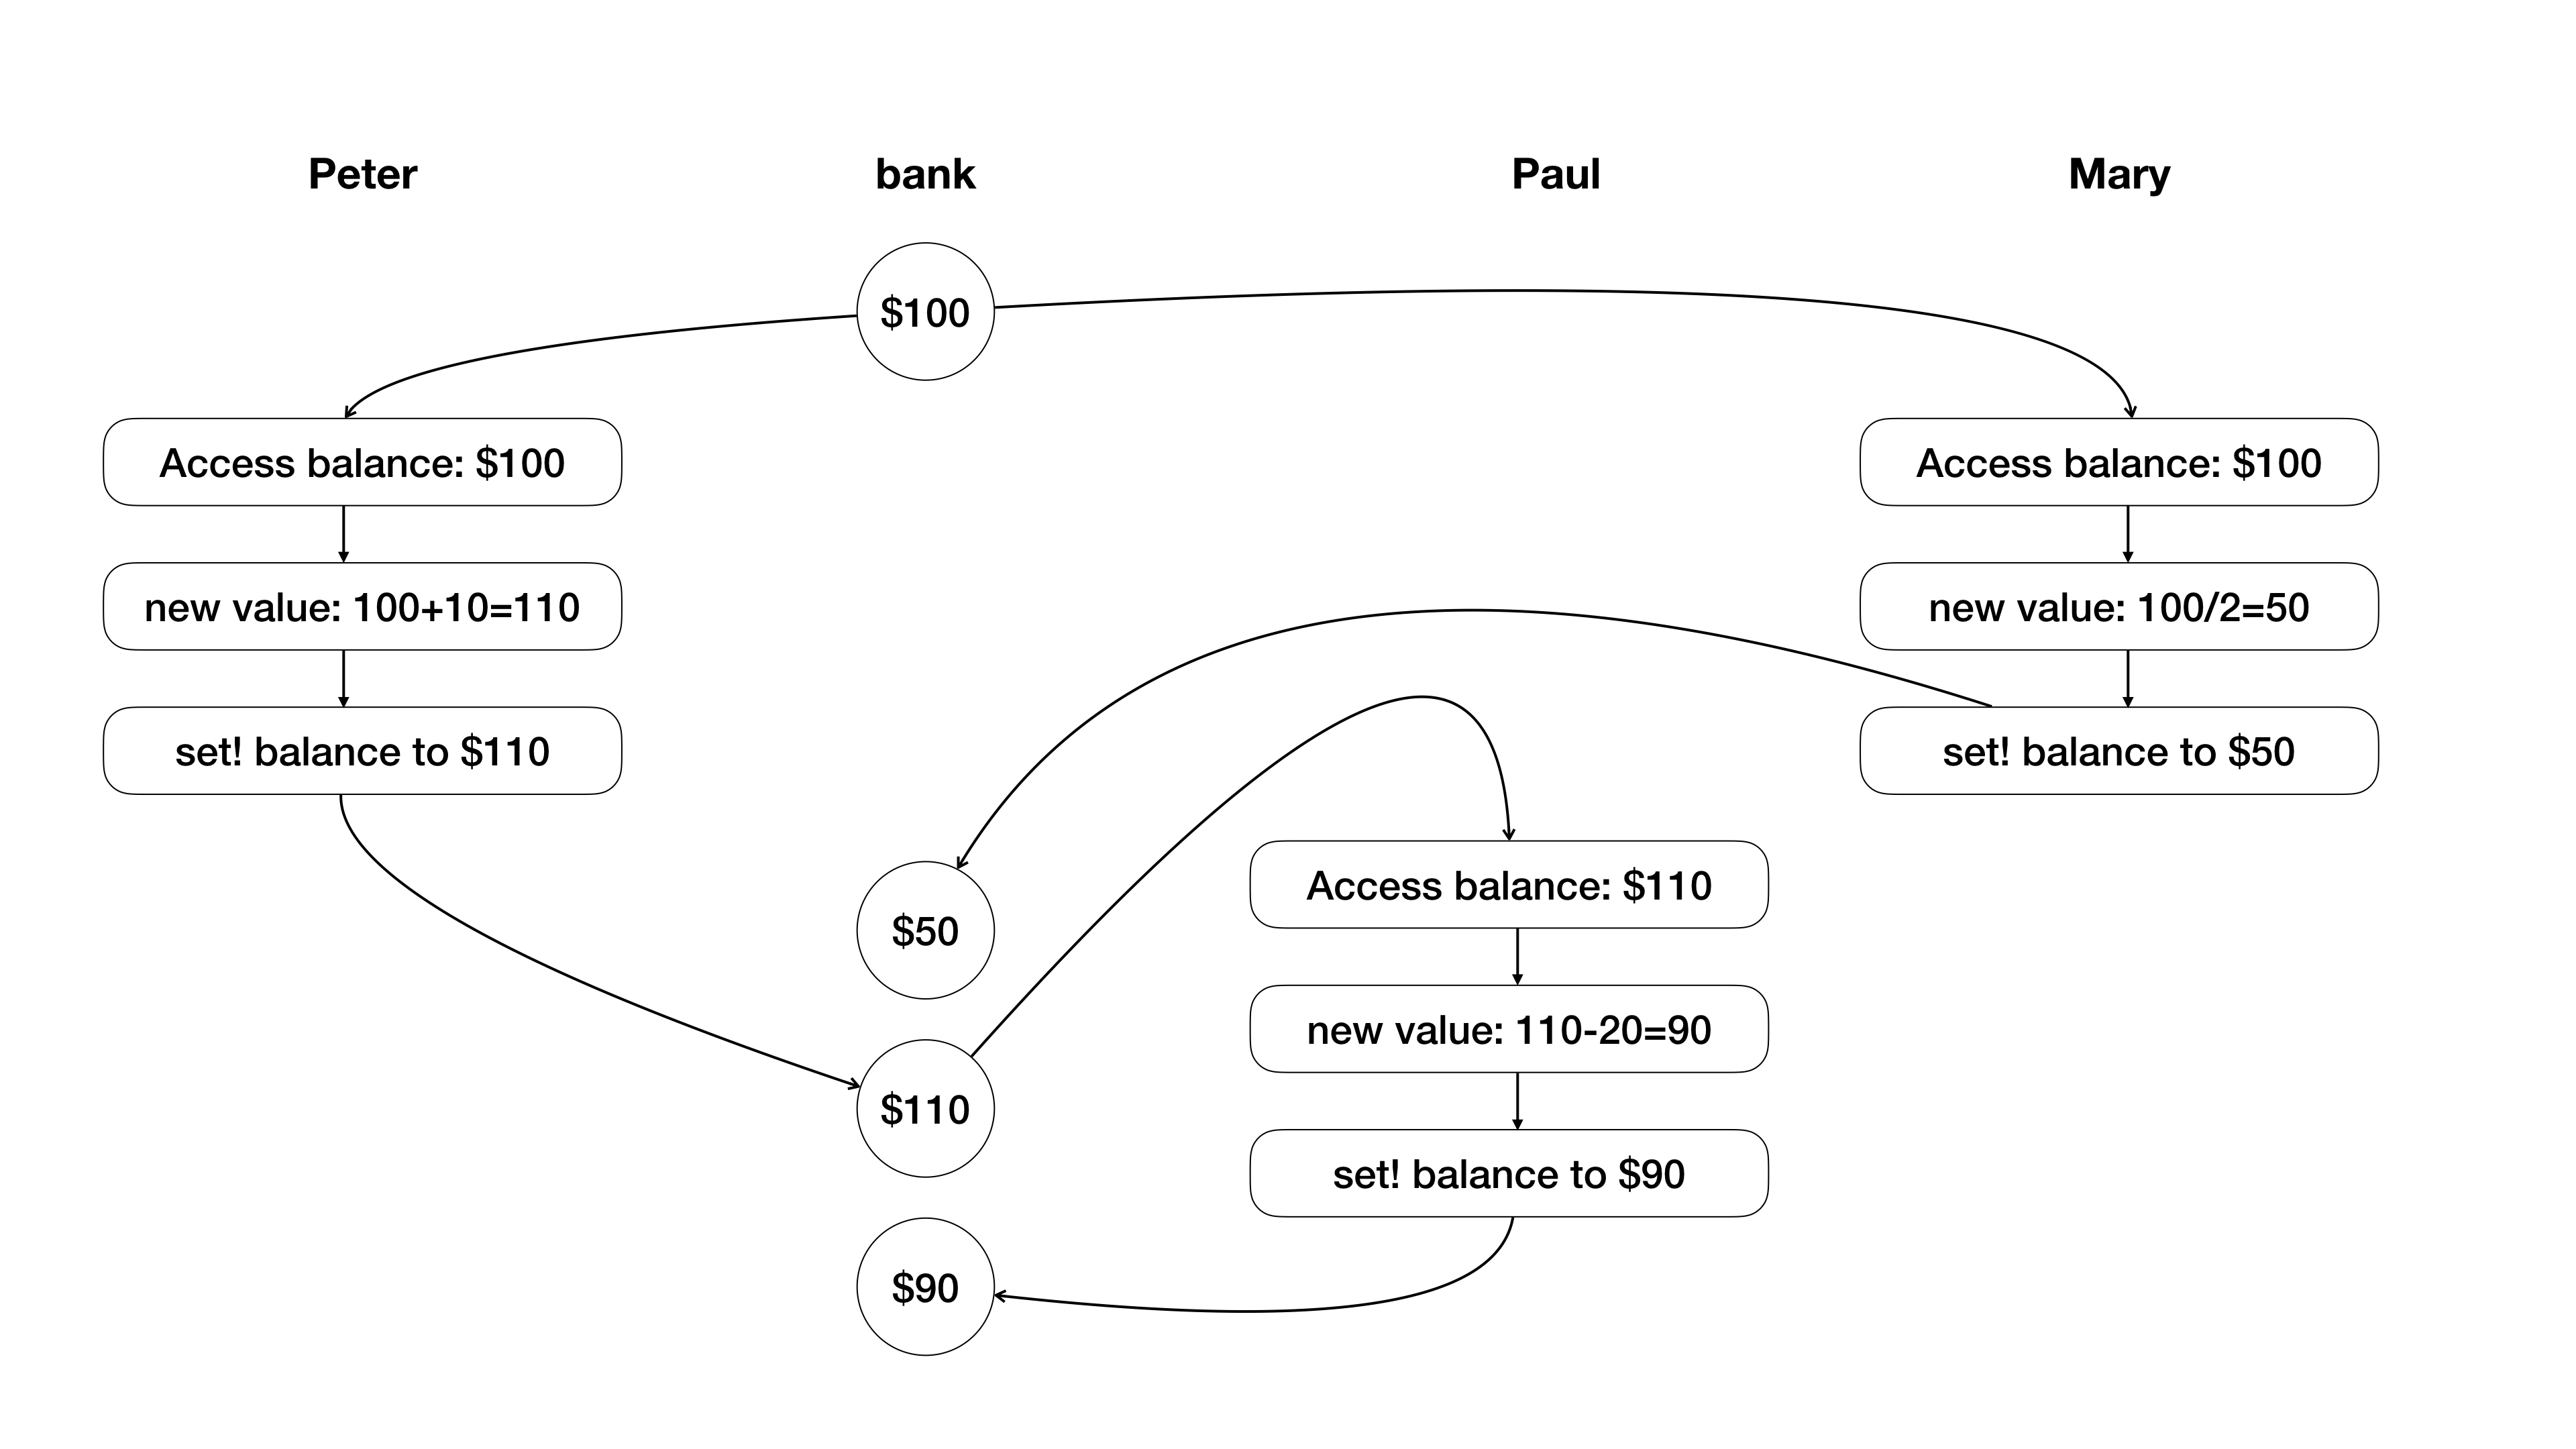
\includegraphics[width=.8\textwidth,height=.8\textheight,keepaspectratio]{5.png}
\end{center}

\begin{center}
    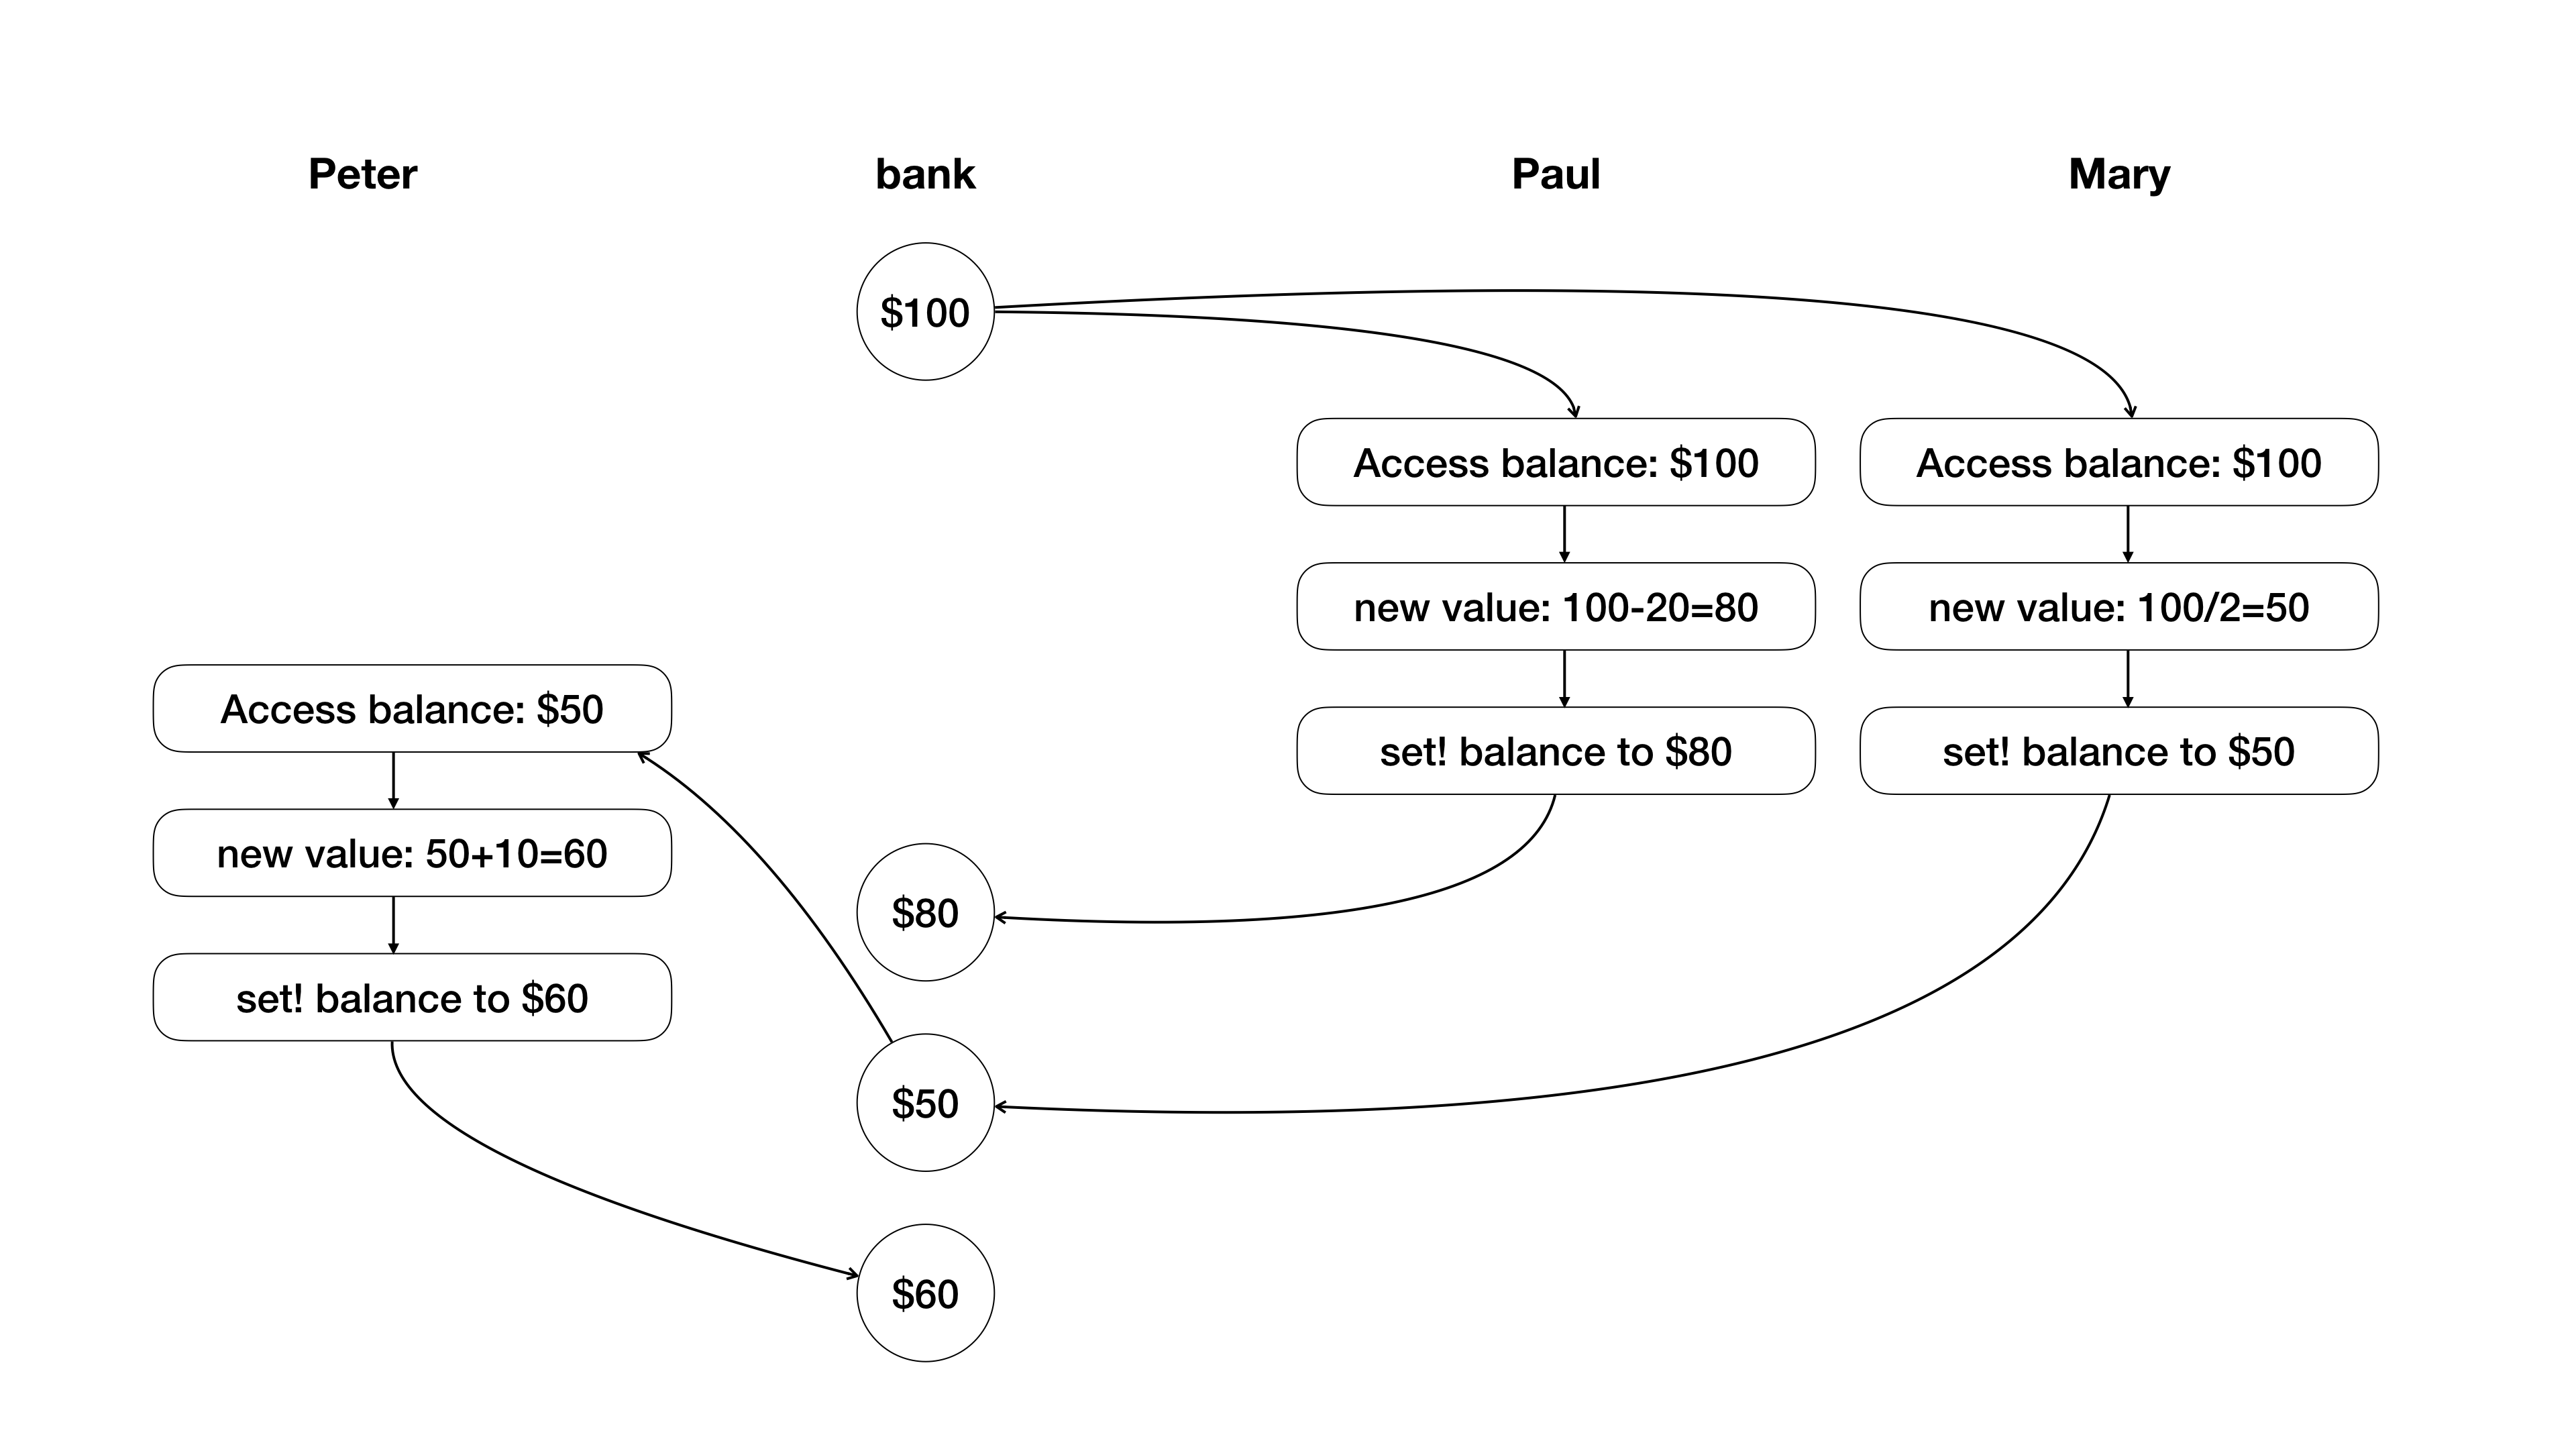
\includegraphics[width=.8\textwidth,height=.8\textheight,keepaspectratio]{6.png}
\end{center}

\begin{center}
    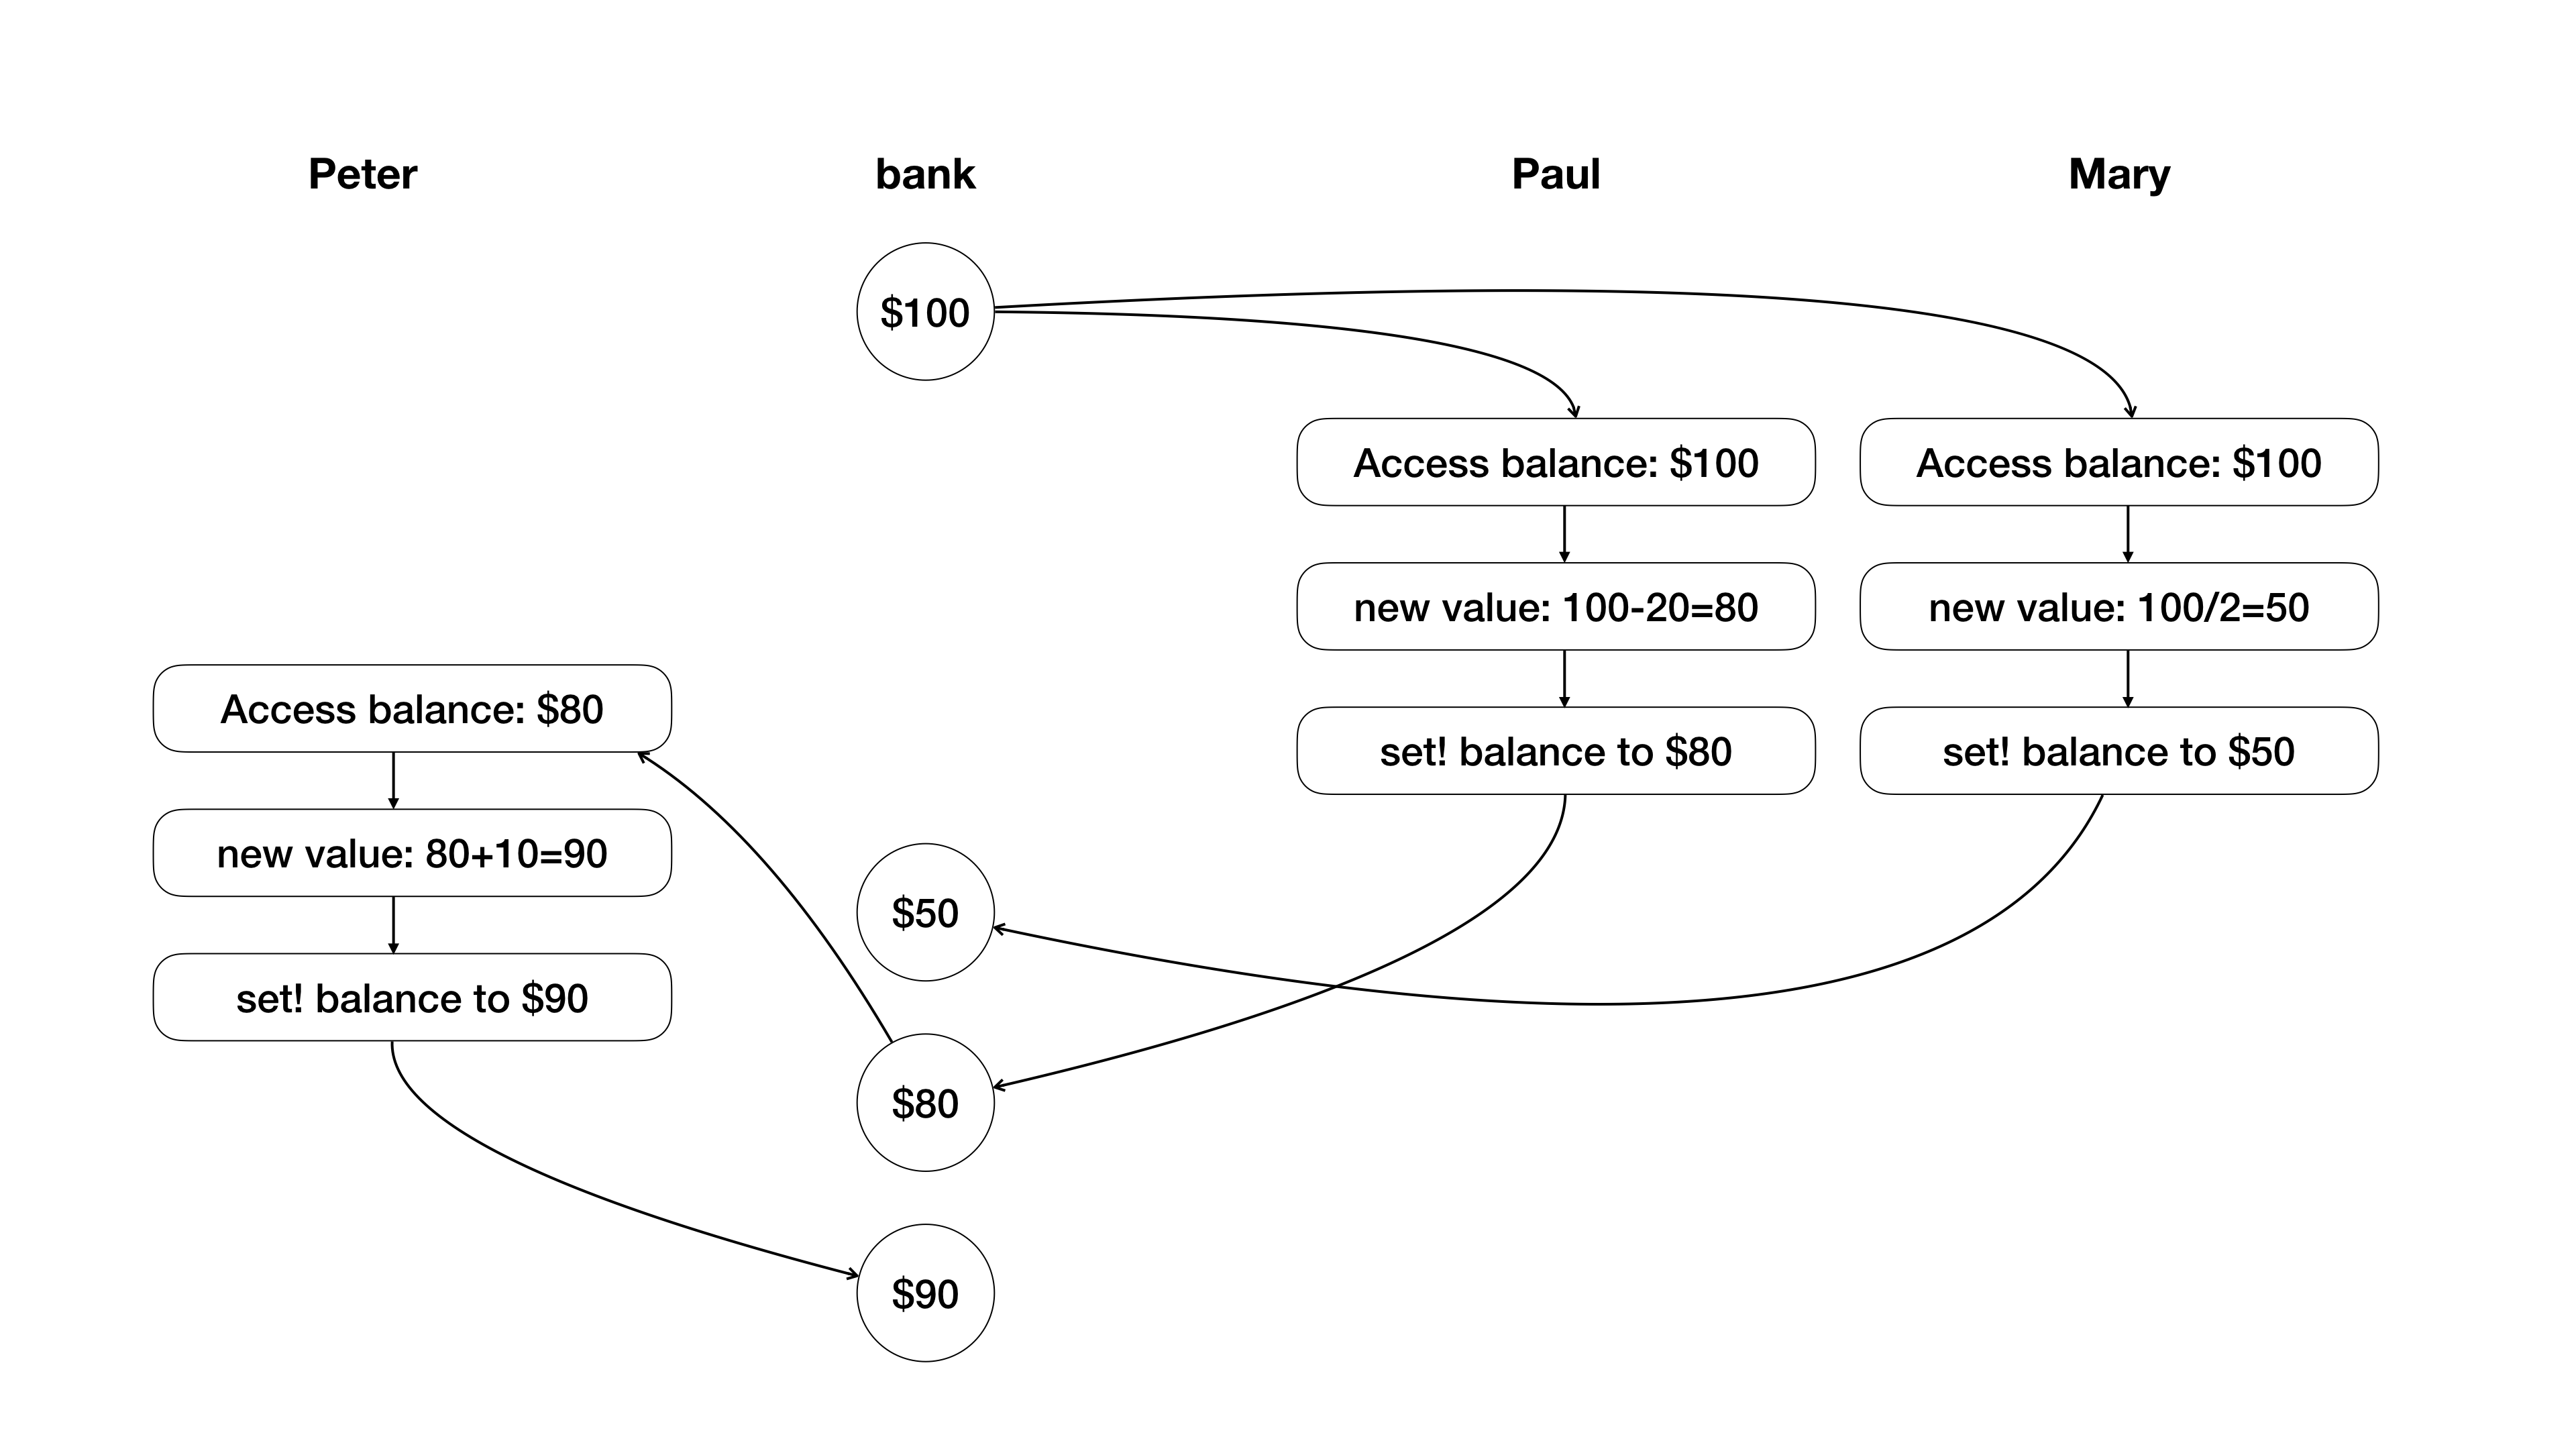
\includegraphics[width=.8\textwidth,height=.8\textheight,keepaspectratio]{7.png}
\end{center}

\end{document}
